\documentclass[12pt,a4paper]{article}
\title{%
  Øving 3 \\
  \large IELET1002 - Datateknikk \\
  }
\author{Gunnar Myhre, BIELEKTRO}

\usepackage[utf8]{inputenc}
\usepackage[norsk]{babel}
\usepackage[siunitx]{circuitikz}
\usepackage{karnaugh-map}
\graphicspath{ {./images} }

\usepackage{color}
\newcommand{\R}{\color{red}}

\newcommand{\N}{\overline}
\setlength\parindent{0pt}

\begin{document}
  \maketitle
  
  \section{Oppgåve 1}
    \subsection{a)}
      Sekvenskoplinga er synkron sidan vippene har det same klokkesignalet, og
      sidan utgongsvariabelen $y$ er kun ein funksjon av vippeutgongane og
      ikkje den eksterne inngongsvariablen $x$ er det snakk om MOORE-logikk
    \subsection{b)}
      Finner først funksjonsuttrykk ved å analysere den kombinatoriske blokka
      \begin{itemize}
        \item $J_A(A,B,x) = \N{A+\bar{B}} \rightarrow \bar{A}B$
        \item $K_A(A,B,x) = \N{ \N{A+\bar{B}} + \N{B+x}} \rightarrow (A+\bar{B})(B+x)
          \rightarrow B\bar{x} + AB$
        \item $J_B(A,B,x) = K_A(A,B,x) = B\bar{x} + AB$
        \item $K_B(A,B,x) = \N{\bar{x} + \bar{B}} \rightarrow Bx$
        \item $y(A,B) = \N{A + B} \rightarrow \bar{A}\bar{B}$
      \end{itemize}
      Finner karakteristisk tabell for JK-vippe
      \begin{center}
        \begin{tabular}{ |c|c|c c| }
          \hline
          $J$ & $K$ & $Q_{t+1}$ & \\
          \hline
          0 & 0 & $Q_t$ & (uendra) \\
          \hline
          0 & 1 & $0$ & (reset) \\
          \hline
          1 & 0 & $1$ & (set) \\
          \hline
          1 & 1 & $Q_{t+1}$ & (toggle) \\
          \hline
        \end{tabular}
      \end{center}
      Så setter eg inn i tabell for tilstand og nestetilstand
      \begin{center}
        \begin{tabular}{ |c| c|c|c|c| c|c| c| }
          \hline
          $ABx$ & $J_A$ & $K_A$ & $J_B$ & $K_B$ & $A_{t+1}$ & $B_{t+1}$ & $y$ \\
          \hline
          000 & 0 & 0 & 0 & 0 & 0 & 0 & 1 \\
          \hline
          001 & 0 & 1 & 1 & 0 & 0 & 1 & 1 \\
          \hline
          010 & 1 & 0 & 0 & 0 & 1 & 1 & 0 \\
          \hline
          011 & 1 & 0 & 0 & 1 & 1 & 0 & 0 \\
          \hline
          100 & 0 & 0 & 0 & 0 & 1 & 0 & 0 \\
          \hline
          101 & 0 & 1 & 1 & 0 & 0 & 1 & 0 \\
          \hline
          110 & 0 & 1 & 1 & 0 & 0 & 1 & 0 \\
          \hline
          111 & 0 & 1 & 1 & 1 & 0 & 0 & 0 \\
          \hline
        \end{tabular}
      \end{center}
    \subsection{c)}
      Teikner tilstandsdiagrammet med dei fire tilstandane $AB$.
      \begin{center}
        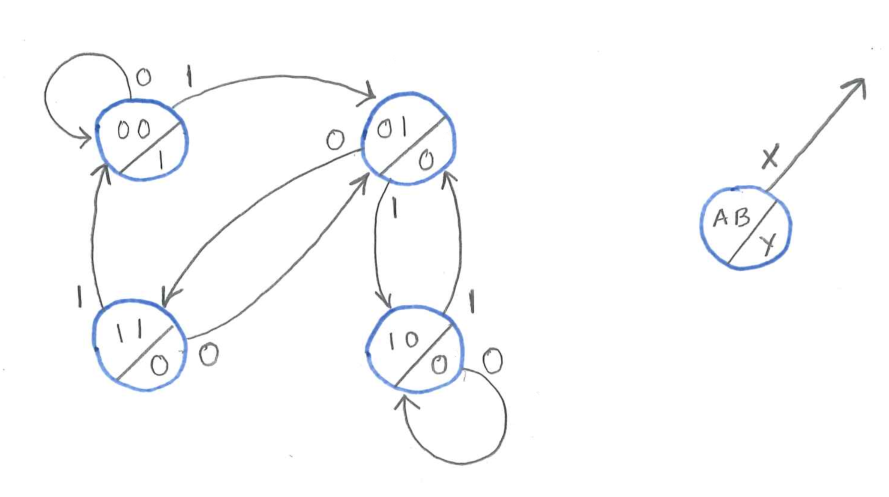
\includegraphics[width=83mm]{04_1c}
      \end{center}
      Dette konkluderer analysen.


  \section{Oppgåve 2}
    \subsection{a)}
      Vi har tre tilstandar, og treng derfor to vipper sidan $2^2 > 3$.
      Setter opp eksitasjonstabell for JK-vippe.
      \begin{center}
        \begin{tabular}{ |c|c|c| }
          \hline
          $Q_T$ & $Q_{t+1}$ & $JK$ \\
          \hline
          0 & 0 & 0X \\
          \hline
          0 & 1 & 1X \\
          \hline
          1 & 0 & X1 \\
          \hline
          1 & 1 & X0 \\
          \hline
        \end{tabular}
      \end{center}
      Fyller inn nestetilstandstabellen med informasjon frå tilstandsdiagrammet
      og vippefunksjonane vha. eksitasjonstabellen til JK-vippe
      \begin{center}
        \begin{tabular}{ |c |c| c|c|c|c| c|c| c| }
          \hline
          Indeks & $ABx$ & $A_{t+1}$ & $B_{t+1}$ & $y$ & $J_A$ & $K_A$ & $J_B$ & $K_B$ \\
          \hline
          0 & 000 & 0 & 0 & 0 & 0 & x & 0 & x \\
          \hline
          1 & 001 & 0 & 1 & 0 & 0 & x & 1 & x \\
          \hline
          2 & 010 & 0 & 0 & 1 & 0 & x & x & 1 \\
          \hline
          3 & 011 & 1 & 0 & 0 & 1 & x & x & 1 \\
          \hline
          4 & 100 & 0 & 0 & 0 & x & 1 & 0 & x \\
          \hline
          5 & 101 & 1 & 0 & 1 & x & 0 & 0 & x \\
          \hline
          6 & 110 & - & - & - & x & x & x & x \\
          \hline
          7 & 111 & - & - & - & x & x & x & x \\
          \hline
        \end{tabular}
      \end{center}
      Tilstanden når $AB = 11$ er ikkje brukt i tilstandsdiagrammet, derfor kan
      vi bruke desse valfrie kombinasjonane til å forenkle logikken. Finner
      vippeinngongsfunksjonane vha. Karnaugh-diagram:
      \begin{center}
        \begin{karnaugh-map}[4][2][1][$Bx$][$J_A(A,B,x) \rightarrow A$]
          \minterms{3}
          \maxterms{0,1,2}
          \indeterminants{4,5,6,7}
          \implicant{3}{7}
        \end{karnaugh-map}
      \end{center}
      $J_A(A,B,x) = Bx$
      \begin{center}
        \begin{karnaugh-map}[4][2][1][$Bx$][$K_A(A,B,x) \rightarrow A$]
          \minterms{4}
          \maxterms{5}
          \indeterminants{0,1,2,3,6,7}
          \implicantedge{0}{4}{2}{6}
        \end{karnaugh-map}
      \end{center}
      $K_A(A,B,x) = \bar{x}$
      \begin{center}
        \begin{karnaugh-map}[4][2][1][$Bx$][$J_B(A,B,x) \rightarrow A$]
          \minterms{1}
          \maxterms{0,4,5}
          \indeterminants{2,3,6,7}
          \implicant{1}{3}
        \end{karnaugh-map}
      \end{center}
      $J_B(A,B,x) = A\bar{x}$
      \begin{center}
        \begin{karnaugh-map}[4][2][1][$Bx$][$K_B(A,B,x) \rightarrow A$]
          \minterms{2,3}
          \maxterms{}
          \indeterminants{0,1,4,5,6,7}
          \implicant{0}{6}
        \end{karnaugh-map}
      \end{center}
      $K_B(A,B,x) = 1$
      \begin{center}
        \begin{karnaugh-map}[4][2][1][$Bx$][$y(A,B,x) \rightarrow A$]
          \minterms{2,5}
          \maxterms{0,1,3,4}
          \indeterminants{6,7}
          \implicant{2}{6}
          \implicant{5}{7}
        \end{karnaugh-map}
      \end{center}
      $y(A,B,x) = B\bar{x} + Ax$
      \begin{center}
        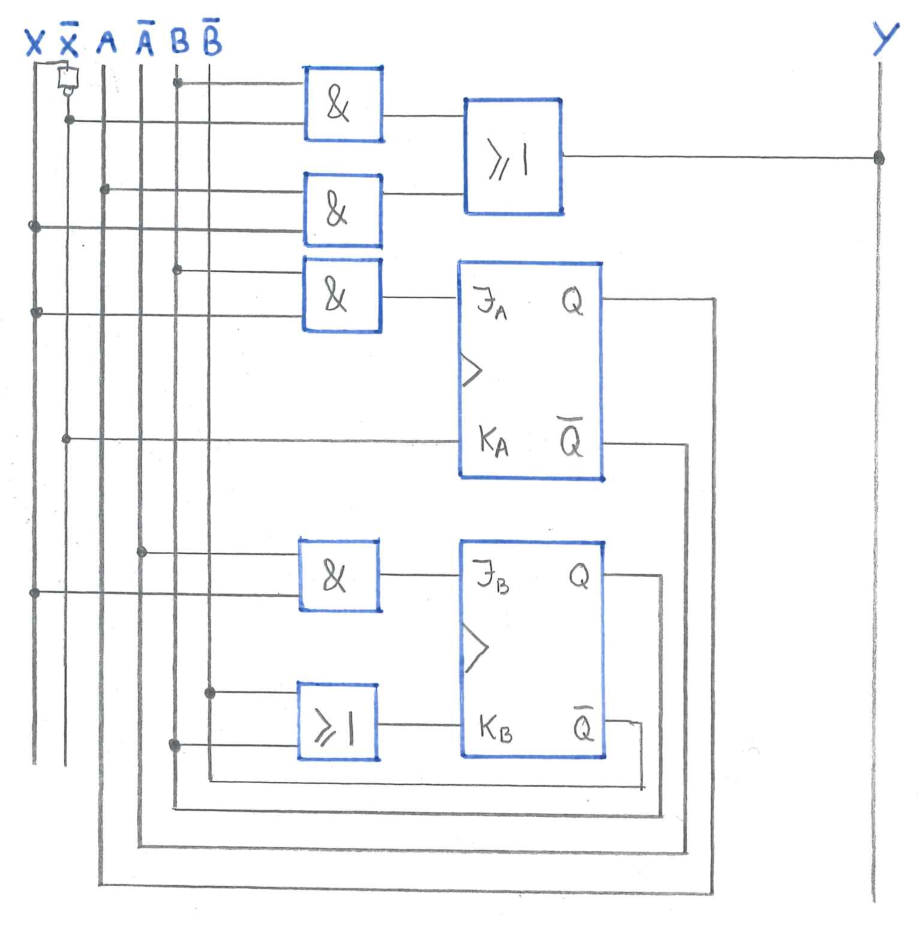
\includegraphics[width=83mm]{04_2a}
      \end{center}
      Med alle funksjonsuttrykka kan vi konstruere den kombinatoriske blokka
      og dette konkluderer konstruksjonen.

    \subsection{b)}
      I forenklinga av funksjonsuttrykka i deloppgåve a) har eg vald verdiar
      for dei valfrie kombinasjonane. Desse kan eg nå fylle inn i
      nestetilstandstabellen.
      \begin{itemize}
        \item $J_A(A,B,x) = \Sigma(3,7)$
        \item $K_A(A,B,x) = \Sigma(0,2,4,6)$
        \item $J_B(A,B,x) = \Sigma(1,3)$
        \item $K_B(A,B,x) = 1$
        \item $y(A,B,x) = \Sigma(2,5,6,7)$
      \end{itemize}
      
      \begin{center}
        \begin{tabular}{ |c |c| c|c|c|c| c|c| c| }
          \hline
          Indeks & $ABx$ & $A_{t+1}$ & $B_{t+1}$ & $y$ & $J_A$ & $K_A$ & $J_B$ & $K_B$ \\
          \hline
          0 & 000 & 0 & 0 & 0 & 0 & \R{1} & 0 & \R{1} \\
          \hline
          1 & 001 & 0 & 1 & 0 & 0 & \R{0} & 1 & \R{1} \\
          \hline
          2 & 010 & 0 & 0 & 1 & 0 & \R{1} & \R{0} & 1 \\
          \hline
          3 & 011 & 1 & 0 & 0 & 1 & \R{0} & \R{1} & 1 \\
          \hline
          4 & 100 & 0 & 0 & 0 & \R{0} & 1 & 0 & \R{1} \\
          \hline
          5 & 101 & 1 & 0 & 1 & \R{0} & 0 & 0 & \R{1} \\
          \hline
          6 & 110 & \R{0} & \R{0} & \R{1} & \R{0} & \R{1} & \R{0} & \R{1} \\
          \hline
          7 & 111 & \R{1} & \R{0} & \R{1} & \R{1} & \R{0} & \R{0} & \R{1} \\
          \hline
        \end{tabular}
      \end{center}
      Ut ifrå denne tabellen kan vi teikne eit nytt tilstandsdiagram som
      inkluderer tilstanden $AB = 11$
      \begin{center}
        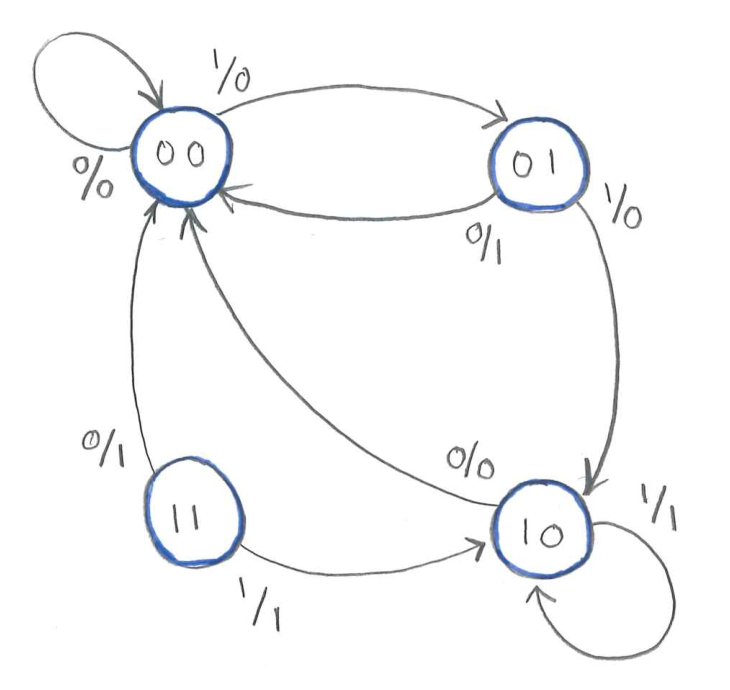
\includegraphics[width=83mm]{04_2b}
      \end{center}
      Sekvenskoplinga er sjølvstartande sidan den kjem over til ein lovleg
      tilstand etter endelig mange periodar (her éin eller to klokkesyklusar,
      avhengig av påtrykt x ved oppstart). Det hadde kanskje vore meir heldig
      om den uønska tilstanden $11$ hadde pekt til $00$ for begge $x$, og at
      den ikkje hadde påtrykt $y=1$.  Korvidt dette er eit problem kjem an på
      kva kretsen skal styre. \bigskip

      Dersom $11$ hadde pekt på seg sjølv for éin verdi $x$ ville kretsen vore
      vilkårleg sjølvstartande. Dette trenger ikkje å vere eit problem (f.eks.
      dersom $x=0$ er default-påtrykket og peker til ein gyldig tilstand).
      \bigskip

      Dersom $11$ hadde pekt på seg sjølv for begge verdiar $x$ ville ikkje
      kretsen vore sjølvstartande. Dette er ikkje bra sidan kretsen i dette
      tilfellet vil henge seg opp dersom den startar i tilstanden $11$.
      \bigskip

      I begge tilfella vil vi kunne endre den kombinatoriske blokka ved å sette
      $11 \rightarrow 00$ som eit kriterie i nestetilstandstabellen og
      konstruere tilstandsdiagrammet på nytt. Men det er verdt å merke seg at
      den kombinatoriske blokka vi har konstruert vha. Karnaugh-diagrammer er
      den enklaste moglege, og krever derfor færrast logiske portar.

      \newpage

  \section{Oppgåve 3}
    \subsection{a)}
      Ein måte å implementere dette på er med fire tilstandar, ein for kvar
      bit i bitmønsteret. Tilstandsdiagram for MEALY-logikk:
      \begin{center}
        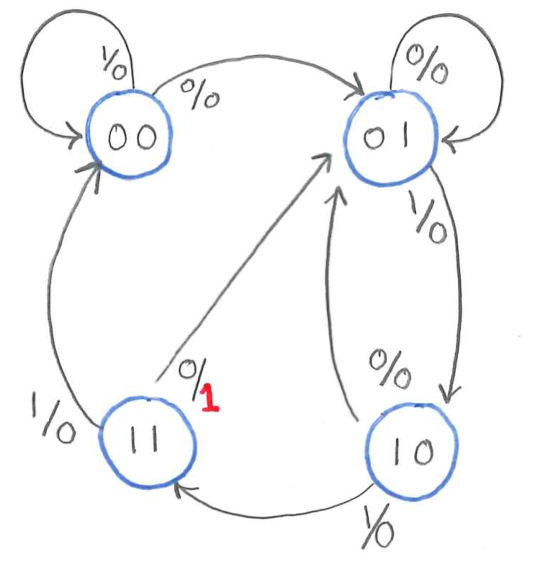
\includegraphics[width=83mm]{04_3a}
      \end{center}
      Ved påtrykk av $0110$ vil ein bevege seg frå tilstand $00$ med klokka, og
      til slutt påtrykke $y$ etter fire riktige påtrykk. Dersom feil $x$ er
      påtrykt vil vi returnere til enten $01$ (om ein $1$ var venta) eller $00$
      (om ein $0$ var venta).

      \newpage 

    \subsection{b)}
      Dette er eit forsøk på å implementere med MOORE-logikk. Eg kan ikkje finne
      nokon måte å gjere dette på med færre enn fem tilstandar.
      \begin{center}
        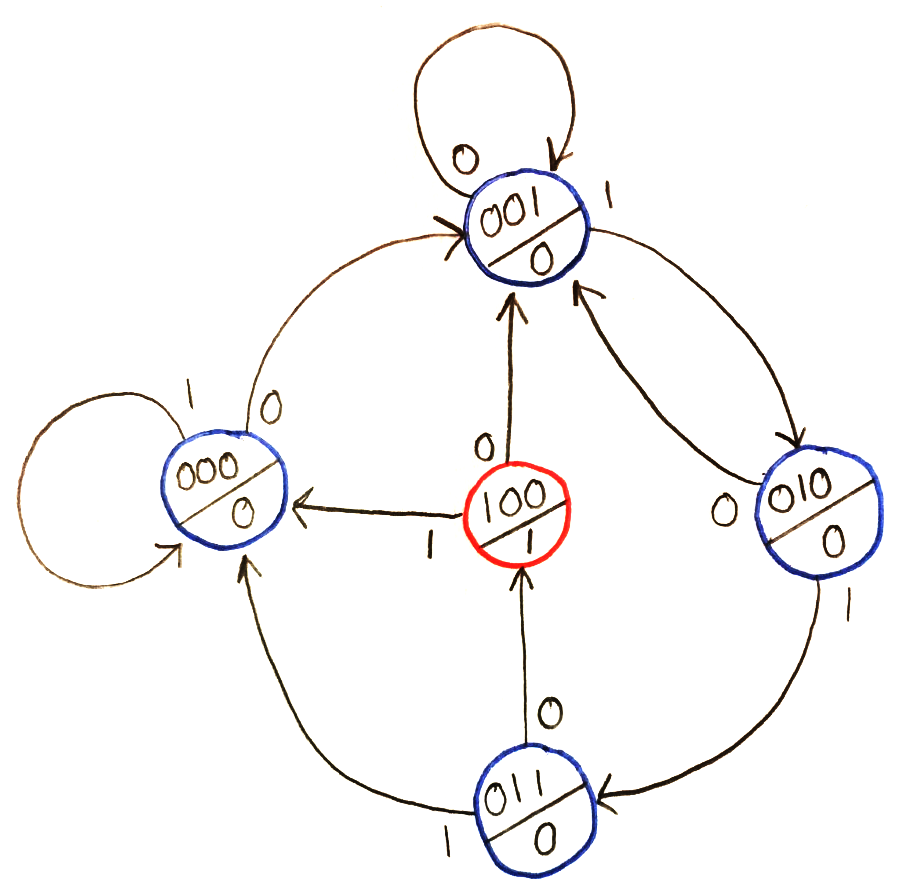
\includegraphics[width=73mm]{04_3b}
      \end{center}
      Kretsen oppfører seg for det meste likt som kretsen i deloppgåve a).
      Forskjelen er at vi har ein ekstra tilstand som kun førekommer dersom
      sekvensen har vorte korrekt påtrykt.

    \subsection{c)}
      Fordelar og ulemper med MOORE-logikk:
      \begin{itemize}
        \item Vi trenger fem tilstandar, og derfor tre vipper. Dette medfører
          fleire komponent i den kombinatoriske blokka (som igjen medfører
          høgare tidsforsinking, høgare energiforbruk og større sjangs for
          feil).
        \item Vi har $2^3 - 5 = 3$ ubrukte tilstandar som potensielt må takast
          hensyn til.
        \item Fordelen er at utgongane er synkrone sidan $y$ er ein direkte
          utgong frå ei vippe. Utgongsverdien vil også ligge fast ein heil
          klokkeperiode.
      \end{itemize}
      Fordelar og ulemper med MEALY-logikk:
      \begin{itemize}
        \item Kretsen har fire tilstandar, så vi trenger kun to vipper.
        \item Utgongen kan reagere straks på endring av inngongsvariabel.
        \item Det er ei ulempe at utgongssignalet kan ha ei levetid som er
          kortare enn klokkesignalet.
      \end{itemize}
      

\end{document}
